% !TeX spellcheck = fr_FR
\documentclass[final, a4paper, 11pt]{article}
\usepackage[french]{babel}
\usepackage[utf8]{inputenc}
\usepackage[T1]{fontenc}
\usepackage{fontspec}
\usepackage{fullpage}
\usepackage{float}
\usepackage[margin=2cm]{geometry}

\begin{document}
\noindent
\large\textbf{Processus « Gestion des Incidents »} \hfill \textbf{KOCAK Mikail} \\
\normalsize M. Jean Martin \hfill 21 novembre 2018

\section{Introduction}

L'objectif de la gestion des incidents est d'instaurer un processus qui
permet au service de retourner à son état de fonctionnement dit
'normal' ; c'est-à-dire, fonctionnant bien dans le cadre défini.

\section{Les informations à être visibles}

Dans la fiche d'incident, les informations suivantes doivent être visibles :

\begin{itemize}
    \item La date courante (assignée automatique) de chaque changement de statut
        (mise en triage, ouverture, escalades, etc.) ;
    \item Un identifiant unique automatiquement associé à l'incident,
        permettant la gestion a travers une infrastructure et le référencement
        entre incidents en relation ;
    \item La catégorie de l'incident (avoir des sous-catégories, 
        de préférence), permettant de filtrer et d'assigner l'incident directement
        au service concerné ;
    \item L'appareil (système d'exploitation, navigateur, nom de la machine, ...) ;
    \item La version si applicable ;
    \item Les étapes pour reproduire (si applicable) ;
    \item La priorité de l'incident ;
    \item Le niveau d'impacte de l'incident ;
    \item Le ou les services impactés
        (machine locale, un service donné, un système donné, ...) ;
    \item Le status de l'incident (voir la section \ref{S:status}) ;
    \item Personne(s) assigné-e-s ;
    \item Le nom de l'utilisateur et ses informations de contact
        (téléphone, courriel, bureau, etc.) ;
    \item Problèmes connus/ résolus en relation.
\end{itemize}

\begin{figure}[H]
    \centering
    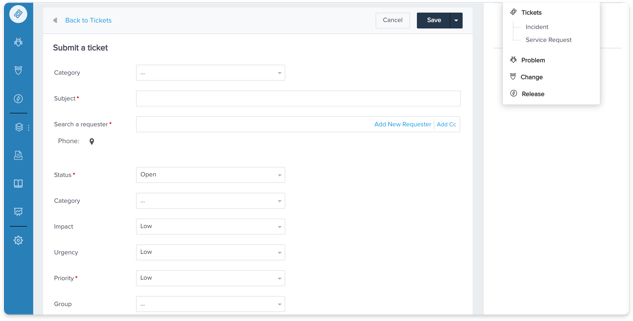
\includegraphics[width=.864\linewidth]
    {assets/empower-employees-with-self-service-5a1a79af.png}
    \caption{Exemple d'interface regroupant les différentes informations requises}
\end{figure}

\section{Les différents statuts}
    \label{S:status}
    \begin{description}
        \item[En attente,] l'incident n'a pas encore été confirmé
            ou n'a pas pu être reproduit, 
            ou il y a un manque d'information.
        \item[Ouvert,] un incident a été reconnu mais n'est pas
            encore assigné à quelqu'un pour une résolution.
        \item[En cours,] l'incident est processus d'investigation
            et de résolution.
        \item[Résolu,] une résolution a été mise en place mais
            la restauration de l'état des services n'a pas encore
            été validée par l'organisme et l'utilisateur final.
        \item[Fermé,] l'utilisateur final a confirmé que l'incident 
            a bien été résolu et que les fonctionnement normal des 
            services a bien été rétabli.
    \end{description}

\section{Priorités}
Il faudrait cibler un temps de résolution en fonction de la priorité,
comme ou relatif à celui cité ci-dessous.

\begin{table}[H]
    \centering
    \begin{tabular}{|c|l|l|}
         \hline
         Code de priorité & Priorité & Temps de résolution cible  \\ \hline
         1 & Critique & 1 heure \\ \hline
         2 & Haute & 8 heures \\ \hline
         3 & Moyenne & 24 heures \\ \hline
         4 & Basse & 48 heures \\ \hline
         5 & Planification & Planifié \\ \hline
    \end{tabular}
    \caption{Temps de résolution cible en fonction de la priorité}
\end{table}


\newpage

\begin{figure}[!htb]
    \centering
    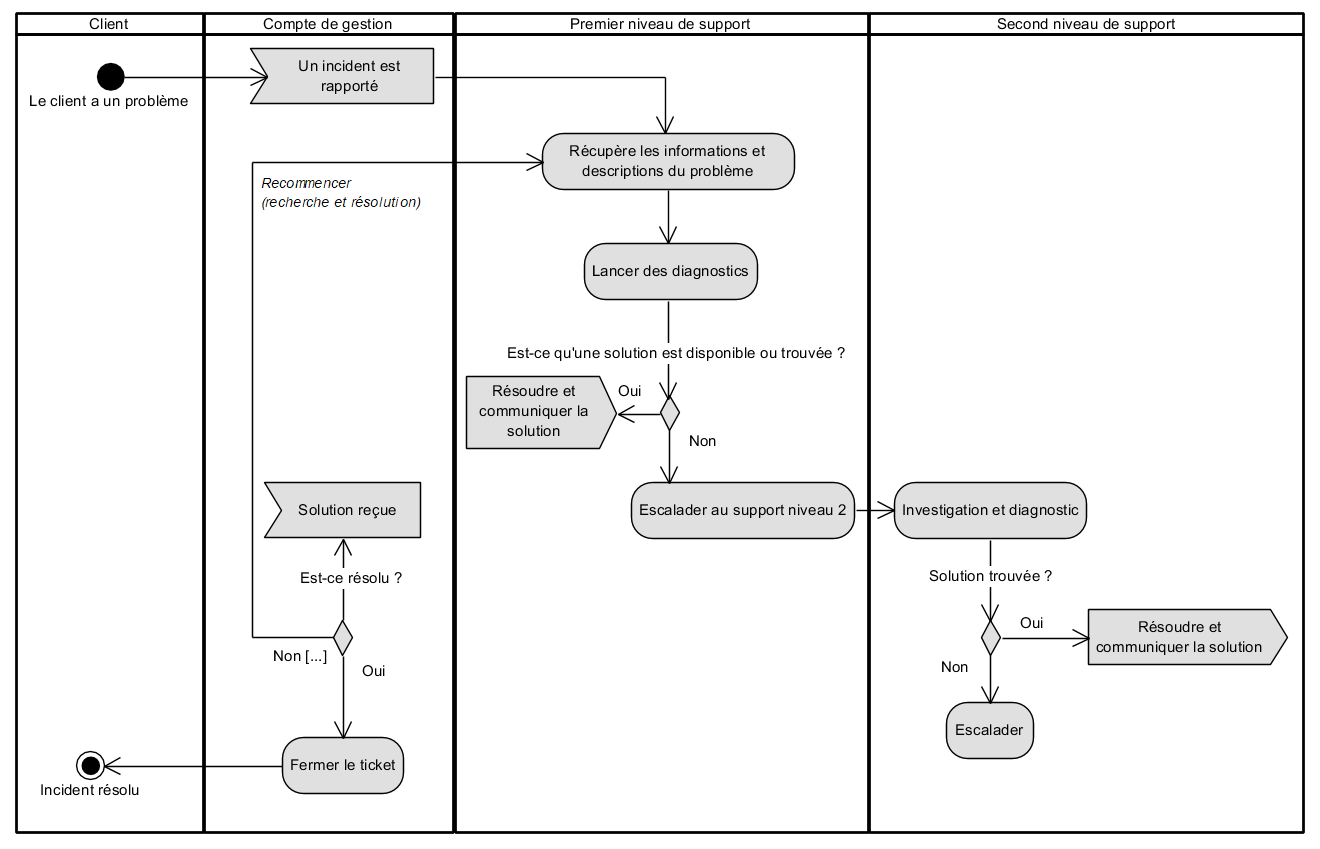
\includegraphics[width=1.44\linewidth,angle=90]{assets/proc_resolution}
    \caption{Simple processus de résolution d'incident.}
\end{figure}

\end{document}
